\documentclass{article}
\usepackage[left=1in,right=1in,top=0.5in,bottom=0.5in]{geometry}
\usepackage{graphicx}
\usepackage{indentfirst}
\usepackage{float}
\setlength\parindent{0pt}
\usepackage{listings}
\usepackage{amsmath}
\usepackage{titletoc}
\usepackage{amsfonts,amssymb}
\usepackage[hyphens,spaces,obeyspaces]{url}
\urlstyle{same}

\begin{document}

\titlecontents{section}[0pt]{\addvspace{4mm}\filright}
{\bfseries\contentspush{\bfseries{\thecontentslabel}\hspace{1.2mm}\ }}
{}{\titlerule*[3pt]{\bf{.}}\hspace*{-0.8em}\bf{\contentspage}}
\newpage
MP1-Cluster Number:g56\\
Yitao HE(Netid:yitaohe2)\\
Tianyu Qiao(Netid:tianyuq2)

\section{Instruction}
\subsection{Library}
To run this Python program, please have those libraries preinstalled:\\
matplotlib.pyplot\\
numpy\\
socket\\
threading\\
selectors\\



\subsection{Command}
Please first have the code cloned into tested VMs and have configFile ready in the folder, the format of configFile is the same as posted in MP1 description, you may want to ensure the number of nodes to connect in each configFile is the same, and there is a match of nodename in command and configFile.\\

Run on machine with command: \\
\url{python3 -u gentx.py [Freq] | python3 simple_client.py [Node_name] [Port] [ConfigFile]} \\

\smallskip\noindent
\url{E.g. python3 -u gentx.py 1 | python3 simple_client.py node1 1234 config_vm1}


\section{Design Document}
\subsection{Building Network}
The network is built to be a decentralized one with P2P connections, (N-1)$^2$ connections are established within a N nodes network.\\
Each node has two threads with one being client(to send messages) and another one being server(to receive messages). Two global variables toSendList and ReceivedList are maintained with other function, with those two threads keeping retrieve(client thread) and append information to them.\\
\subsection{P2P Reliable Connection,TCP}
TCP protocol is used to guarantee FIFO and reliable communication between Node-to-Node(P2P) channels, it is used by directly using socket function in python.
\subsection{Multicast}
With a client thread to send information building on TCP connection, the unicast function between two nodes is automatically fulfilled. If a node wants to multicast to other nodes, it calls the unicast function multiple times to send all other nodes the same message.
\subsection{Data Structure and Message Interpretation}
Messages are packed with other information to be transmitted in the network, it has content:\\
packinfo = type$|$nodeName$|$time$|$priority$|$msg\\
type=0:Message is a request in ISIS algorithm, please respond the proposed priority for this event on receiving\\
type=1:Message is a respond to a request, please update the priority on receiving\\
type=2:the priority is agreed, please update priority and mark as delivered on receiving\\
nodeName is the identifier of sender node\\
Time is the initial time to create this message\\
Priority is the agreed or proposed priority\\
Msg is the content of message\\

Several data structures are maintained as a global variable in the process:\\
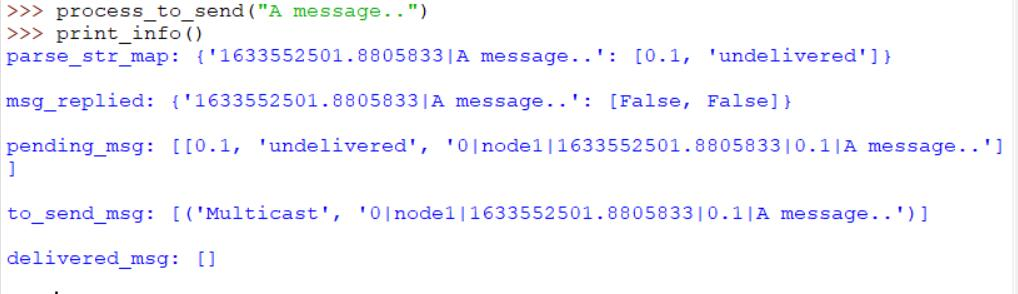
\includegraphics[scale=0.7]{msg.jpg}\\
For example, if a message is sent from me, I would record its time 1633552501.8805833 and the content of message 1633552501.8805833$|$A message, and this serves as the key of two maps, parseStrMap[key] is the priority and delivered status, and msgReplied[key] is whether I have received a proposed priority from other processes. PendingMsg is the queue in ISIS algorithm, and toSendMsg is the message I want to send, deliveredMsg is the message poped out from queue, meaning the message has been delivered.
\subsection{Total Ordering}
Though being expensive, total ordering is used in the network to maintain the same order between different processes. ISIS algorithm is applied in the program.\\
It contains mainly three steps:\\
Sending: a process wants to send a message into the network, it multicast a TYPE0 message.\\
On receiving message with: \\
type=0:Message is a request in ISIS algorithm, please respond the proposed priority for this event on receiving\\
type=1:Message is a respond to a request, please update the priority on receiving, if have received response from all other nodes, multicast the final priority to others(Multicast a TYPE2 msg)\\
type=2:the priority is agreed, please update priority and mark as delivered on receiving\\

\subsection{Failure Handling}
This system can support up to one node failing in the system(assuming it will not be alive again), TCP connection can throw BrokenPipe error when sending message meets a problem. In this case, catch this error and mark this node as unconnected.\\
First, multicast will no longer send message to this node.\\
Second, in the queue of ISIS algorithm, change inside elements, marking it has received response from the failed node.(Otherwise, the front of the queue may never change from undelivered to delivered because it may not receive response from the failed node in the future)\\
Third, whenever receiving a response(proposed priority) in ISIS algorithm, originally we want to mark the info as delivered if have received response from all nodes, now we only want to receive response from other nodes except the failed one.

\section{Graph}
3 nodes, 1Hz, 60 sec can provide following graph\\
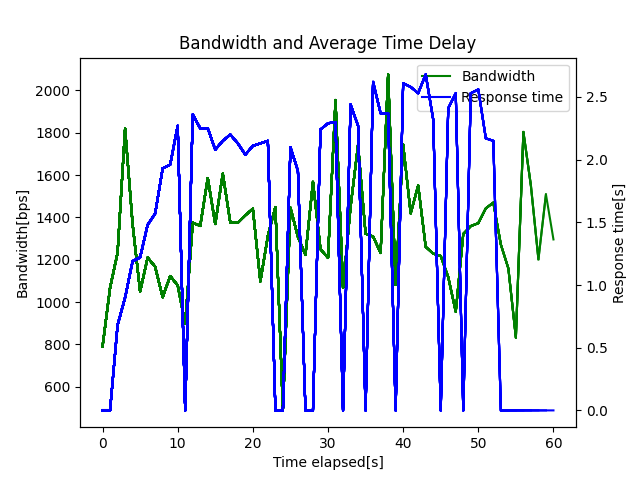
\includegraphics[height=8cm, width=18cm]{60.png}\\


\end{document}